\documentclass[11pt,a4paper,spanish]{book}

\usepackage[spanish,es-tabla]{babel}

\usepackage[utf8]{inputenc}

\usepackage{graphicx}

\usepackage{subcaption}

\usepackage[hidelinks]{hyperref}

\usepackage[a4paper,left=3cm,right=2cm,top=3cm,bottom=2cm]{geometry}

\usepackage{url}

\usepackage{lineno}
\linenumbers

\usepackage{babelbib}

\setlength{\parskip}{1.5mm}

\usepackage{appendix}
\renewcommand{\appendixname}{Anexos}
\renewcommand{\appendixtocname}{Anexos}
\renewcommand{\appendixpagename}{Anexos}

\begin{document}

%Empieza la numeración en números romanos
\frontmatter
% Incluimos la carátula
%Observación: Si bien la página del prefacio dice que sea empty, debería
%comenzar allí la numeración. Se sugiere numeración romana. Recomenzar la
%numeración en el primer capítulo de la tesis con numeración arábiga.

\titlepage

\begin{center}
\ \\
\ \\
\vspace{-1cm}


\ \\

\vspace{0.5cm}
{\Large{\bf \sc Universidad Nacional del Comahue}}\\

\ \\
{\Large { \sc Facultad de Informática}}\\

\vspace{-2.5cm}
\mbox{\hspace{-1cm}\includegraphics[width=2.5cm,height=2.5cm]{logos/unc.png}\hspace{13cm} 
\includegraphics[width=2.5cm,height=2.5cm]{logos/fai.png}}


\vspace{6cm}

{\Large {\bf\sc Tesis de Licenciado en Ciencias de la Computación}}\\
\ \\
\ \\
{\LARGE {\bf Un sistema paralelo de visión global para futbol de robots
	orientado al uso educativo}}\\
\vspace{3cm}

{\Large Autor: Cañibano, Rodrigo S.}\\
\vspace{2cm}

{\Large Director: Balladini, Javier}\\
\ \\
{\Large CoDirector: Grosclaude, Eduardo}\\

\vfill
{\Large {\sc Neuquén}\hspace{6cm}{\sc Argentina}}\\
\ \\

{\Large 2017}\\

\end{center}

\pagebreak



\ \\
\ \\
\label{pagpref}
\noindent{\LARGE \sc Prefacio}\\
\ \\
\ \\

\ \\

\ \\
\ \\


Esta tesis es presentada como parte de los requisitos finales para optar al
grado académico de {\em Licenciado en Ciencias de la Computación}, otorgado por
la Universidad Nacional del Comahue, y no ha sido presentada previamente para la
obtención de otro título en esta Universidad u otras. La misma es el resultado
de la investigación llevada a cabo en el Departamento de ingenieria de
computadoras de la Facultad de Informática, en el período comprendido entre
febrero de 2015 y mayo de 2016, bajo la dirección de Javier Balladini y la
codirección de Eduardo Grosclaude.

\vspace{3cm}


\ \\
{\flushright Rodrigo S. Cañibano\\
{\sc Facultad de Informática \\
Universidad Nacional del Comahue}\\
{\em Neuquén, 25 de mayo de 2016.}\\}

\vfill

\begin{center}
%
\framebox{\begin{minipage}[t]{0.9\columnwidth}%
\begin{flushleft}
\includegraphics[scale=0.035]{logos/unc.png}

\vspace{-2cm}
{\large \hspace{5cm}\sc universidad
nacional del comahue} \\
\par\end{flushleft}
\begin{center}
{\large \qquad{}}{ \hspace{2.5cm} Facultad de Informática}
\par\end{center}

\vspace{1cm}

\indent \ \ \ \ \ \ \ \ \ \ \ La presente tesis ha sido aprobada el día ........................., mereciendo la \\
\indent \ \ \ \  \ \ \ \ \ calificación de .............................

\medskip{}

\vspace{1cm}
\end{minipage}}
\end{center}

\pagebreak


% Incluimos la página de resumen
% vim: set spell spelllang=es syntax=tex :
\ \\
\ \\
\label{pagresum}
\noindent{\LARGE \sc Resumen}\\
\ \\
\ \\

\ \\

\ \\
\ \\
Descripción de la tesis de hasta 500 palabras.\\

 Deberá contener mínimamente motivación,  objetivo, resultado y conclusiones. 

\vfill
\pagebreak


% Incluimos la página de resumen en inglés
% vim: set spell spelllang=en syntax=tex :
\ \\
\ \\
\label{pagsumm}
\noindent{\LARGE \sc Abstract}\\
\ \\
\ \\

\ \\

\ \\
\ \\

The \emph{RoboCup} (short for \emph{Robot World Cup}) is a tournament where two
teams play a simplified version of football. Its aim is to provide a platform
where the advances on multiple fields like artificial intelligence, computer
vision, and robotics can be put to a test. The \emph{RoboCup} has five leagues
ranging from simulated robots on a virtual field, up to humanoid robots with
local vision. Its oldest league is the \emph{Small Size League}, also called the
\emph{SSL}.

On a \emph{SSL} game, the global vision system is shared by both teams. The
system process the video frames and reports the robots' and ball's position and
orientation. We propose an alternative global vision system to that used by the
\emph{RoboCup} for the \emph{SSL} games, that can be used as a learning tool for
computer vision and shared memory parallel programming courses.

For a global vision system to be useful as a learning tool, its detection
algorithms must have a clear conceptual division and be implemented simply so it
can be easily modified (even if it implies a performance loss). Using a base
system, we develop a new system able to efficiently use multiple processing
units and its memory hierarchy. Two parallelization strategies where apply. The
first one applies parallelism inside a frame, dividing the frames into fragments
that are processed independently. The other strategy is based on the
simultaneous precessing of different frames.

The system was implemented using \emph{OpenMP} shared memory programming model
for \emph{C++}. The application's parallelization strategies' parameters can be
tuned to obtain maximum performance for a specific hardware platform. On a
server with an Intel Xeon E5-2630 processor (with 6 processing units and
simultaneous multithreading), we achieve an improvement of 5.42$x$ \emph{FPS},
in comparison to an execution using only one processing unit (from the 6
available). The parallelization strategies can be modified, this can be used to
let students experiment and analyze its results to explain its impact on the
system performance.

\vfill
\pagebreak


\tableofcontents
\listoffigures
%Empieza la numeración en números arábigos
\mainmatter

\chapter{Introducción}

% vim: set spell spelllang=es syntax=tex :

\section{Fútbol de robots}

La \emph{RoboCup}\cite{robocupHist} (del inglés \emph{Robot World Cup}) es una
competencia internacional celebrada desde 1997, donde equipos de robots juegan
una versión simplificada del fútbol. Su finalidad es la de ofrecer un ambiente
controlado donde poner a prueba los avances en distintas áreas de conocimiento
como la inteligencia artificial, visión por computadora y robótica. Existen
cinco ligas distintas cuyas características varían desde la simulación del
ambiente y de los robots, hasta robots humanoides con visión local. De éstas, la
más antigua es la liga de tamaño pequeño (\emph{SSL}, del inglés \emph{Small
Size League}).

Nota de OSO: Se puede agregar info detallada de cada una de las ligas

Un partido de la \emph{SSL} enfrenta a dos equipos de seis robots, que deben
tener un tamaño menor que un cilindro de 9$cm$ de radio y 15$cm$ de
alto\cite{sslrules2015}. Los robots tienen capacidad de procesamiento reducida,
y cada equipo cuenta con una computadora fuera del campo de juego, a la cual se
delega la toma de decisiones. Estas computadoras perciben el ambiente a través
de un sistema de visión global centralizado compartido. Se utiliza un conjunto
de cámaras, montadas sobre distintas áreas del campo de juego y conectadas a una
computadora donde se ejecuta el sistema de visión. El sistema detecta la
posición y orientación de cada uno de los robots y la posición de la pelota, y
reporta esta información a las computadoras que controlan los equipos.

Para que el sistema de visión pueda identificar a cada robot, cada uno tiene
sobre su parte superior cinco parches de colores (Fig. \ref{sistemaVG}). El
parche que se encuentra en el centro indica el color del equipo del robot, y los
cuatro restantes sirven para identificar al robot dentro del equipo y para
conocer la orientación que lleva en cada momento. La pelota es de un color
uniforme y distinto al de los parches de los robots; normalmente, naranja, ya
que este color contrasta fácilmente con el verde de la cancha.

\begin{figure}[!h]

	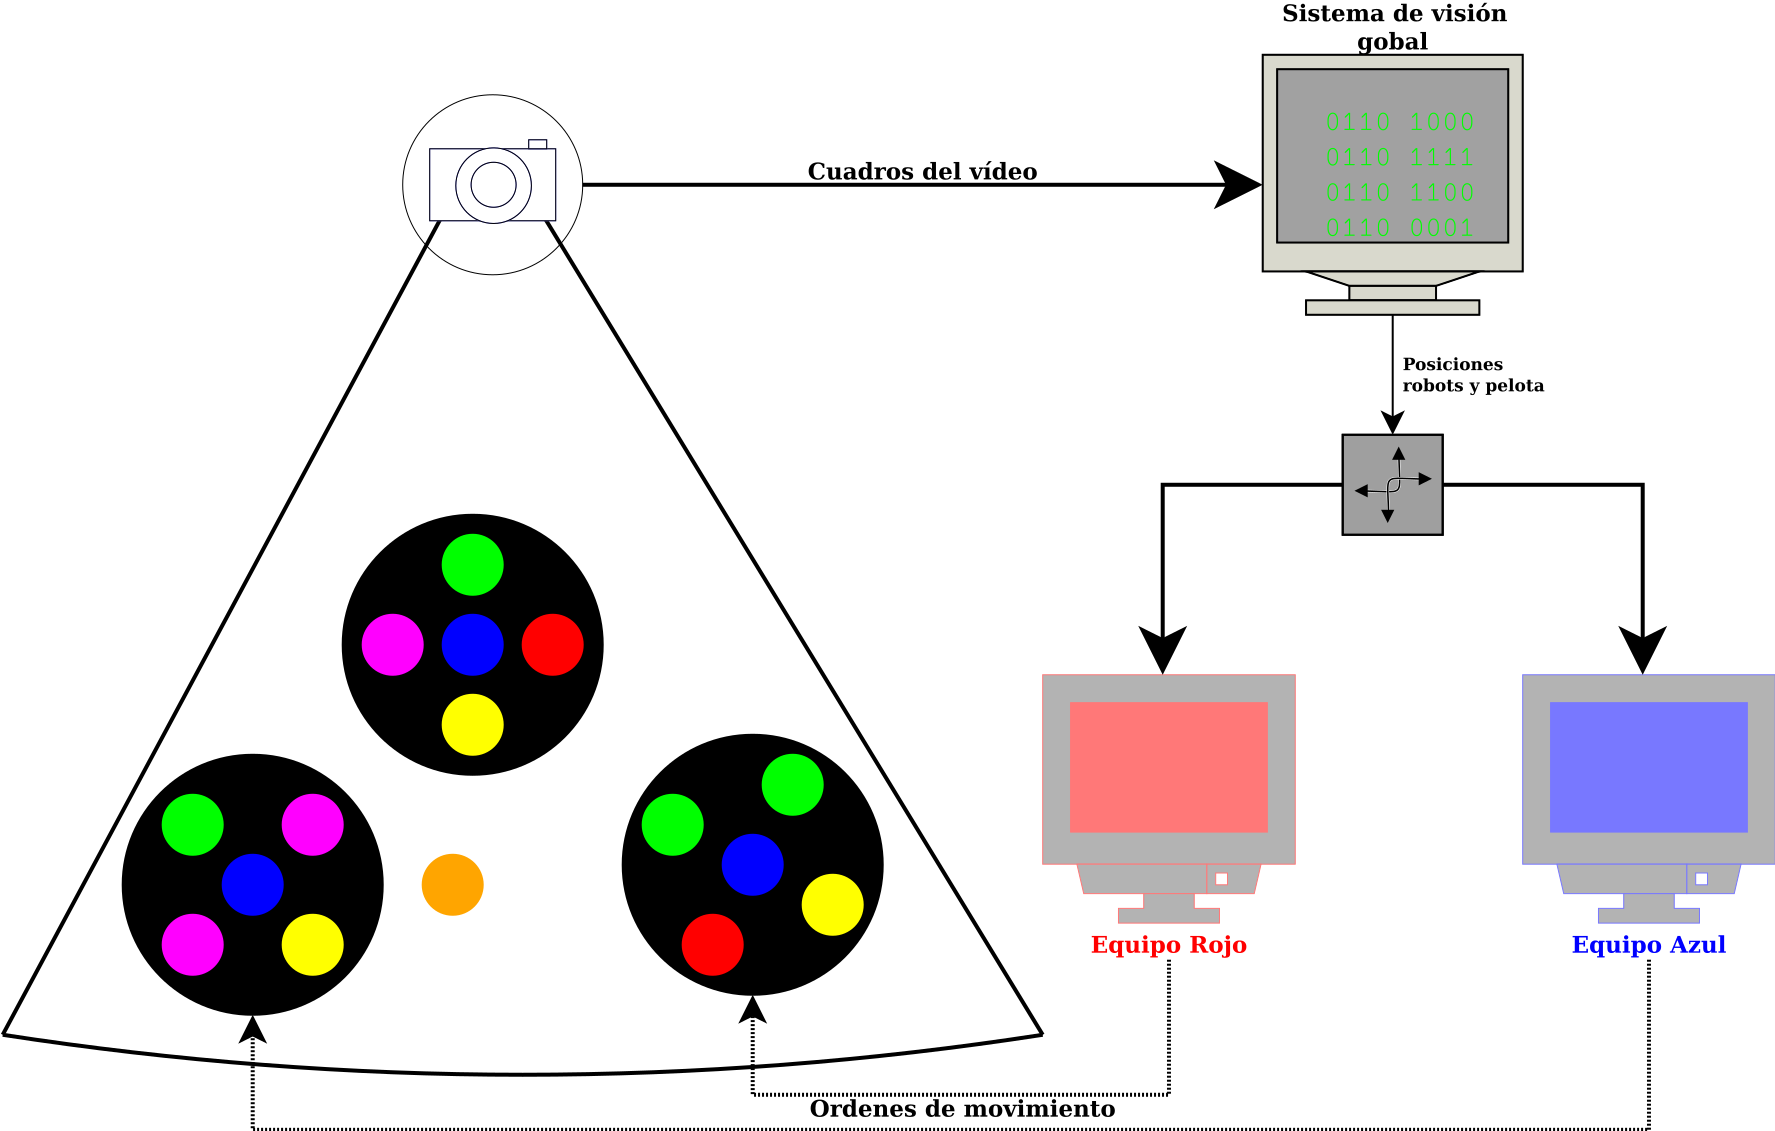
\includegraphics[width=\textwidth]{img/sistemaVG.pdf}

	\caption{Estructura de comunicación del sistema de visión global en
	fútbol de robots de la \emph{SSL}.}

	\label{sistemaVG}

\end{figure}

El uso de este sistema centralizado permite a los participantes abstraerse de
los problemas de la visión por computadora y enfocarse en la estrategia del
juego. Además, permite que las tareas de calibración y montaje de las cámaras se
realicen una sola vez para cada campo de juego, en vez de para cada partido.

Originalmente el tamaño de la cancha era de 4,9$m\times$3,4$m$, lo que permitía
que todo el campo de juego fuera observado con una sola cámara. Luego se optó
por dos tipos de canchas en los partidos de la \emph{SSL}: las canchas de tamaño
simple, con un tamaño de 6,05$m\times$4,05$m$ para las cuales se utilizan dos
cámaras, una sobre cada media cancha, y las de tamaño doble, con un tamaño de
8,09$m\times$6,05$m$, que utilizan cuatro cámaras, una por cada mitad de cada
media cancha (Fig. \ref{FALTA}). Desde el año 2015, las canchas de tamaño doble
son las utilizadas de forma predeterminada\cite{sslrules2015}. Con este cambio
se espera permitir la exploración de nuevas tácticas por parte de los equipos,
ya que una mayor área de juego permite a los robots movimientos de mayor
amplitud y variedad.

\begin{figure}[!h]

	\includegraphics[width=\textwidth]{img/FALTA.png}

	\caption{Dimensiones y área de cobertura de las cámaras en la liga
	\emph{SSL}, en competencias a) anteriores a 2015; b) año 2015 y
	posteriores.}

	\label{FALTA}

\end{figure}

Sin embargo, como consecuencia, en las canchas de tamaño doble, el sistema de
visión debe procesar cuatro veces más información que en las canchas originales;
lo que da lugar a un problema. En efecto, el fútbol de robots se desarrolla en
un contexto de tiempo real, ya que el ciclo completo de procesamiento de
información debe cumplirse en un plazo máximo para poder alcanzar los objetivos.
El servidor debe procesar cada cuadro para entregar la información de posición y
velocidad de cada elemento en el campo de juego a las computadoras coordinadoras
de los equipos; y éstas deben tomar una decisión y comunicarla a los robots,
todo dentro de un tiempo de respuesta razonable para el progreso de la
aplicación.

Los parámetros de calidad de este tipo de sistema son, normalmente:

\begin{itemize}

	\item 	tasa de aciertos en la detección de objetos;

	\item 	precisión en la posición y orientación de los aciertos en la
		detección de objetos;

	\item 	precisión en la posición y orientación de los robots y pelota;

	\item 	cuadros por segundo (\emph{FPS}, del inglés \emph{Frames Per
		Second}) procesados;

	\item 	y máximo tiempo de espera del cuadro (tiempo desde la creación
		del cuadro hasta la entrega de la información extraída).

\end{itemize}

Duplicar la cantidad de información que se debe procesar impacta negativamente
en el rendimiento de estos sistemas, debido a que se reducen los cuadros por
segundo procesados y se incrementa el tiempo de espera del cuadro. Para aumentar
el rendimiento de estos sistemas es necesario implementar soluciones paralelas
que aprovechen las múltiples unidades de procesamiento de las arquitecturas de
cómputo actuales.


% vim: set spell spelllang=es syntax=tex :

\section{Visión por computadora}

La disciplina de Visión por Computadora engloba el estudio de métodos de
captura, mejoramiento, y extracción de información a partir de imágenes. Su
objetivo principal es definir un modelo de una escena a partir de imágenes
\cite{cvLinda2001}. En el caso particular del fútbol de robots, el modelo que se
quiere definir es aquel que describe tanto la posición y orientación de los
robots como la ubicación de la pelota dentro de la cancha. Es un campo con
aplicaciones tan variadas como la identificación de distintas especies de
plantas \cite{plantIdentificacionUCVT2018}, el reconocimiento de bioindicadores
en imágenes \cite{anurosEmImagm2016}, el control de vehículos autónomos
\cite{e2eLearning4SDC} (incluso en otros planetas
\cite{twoYearsMarsRovers2007}), o la aplicación de maquillaje virtual en
fotografías y videos \cite{virtualMakeup2015}.

Los primeros trabajos de visión por computadora fueron realizados durante la
década del 60. En ese momento se consideraba que una aplicación capaz de
describir los elementos de una imagen podía ser desarrollado durante el receso
de verano \cite{summerVisionProject1966}. En la actualidad, gracias a los nuevos
desarrollos en el área de visión por computadora, el incremento en las
capacidades de cómputo, y la disponibilidad de los conjuntos de entrenamiento,
se puede desarrollar un sistema de visión por computadora en un tiempo aun
menor, siempre y cuando se tengan las herramientas indicadas.

La reducción del costo, tamaño y consumo energético de los dispositivos de
captura de imágenes ha permitido que cámaras, GPS y acelerómetros puedan ser
montados con facilidad en una gran variedad de dispositivos, como automóviles,
drones o celulares, o ser llevados por la persona misma o en su ropa,
incrementando la capacidad de captura drásticamente. La proliferación de los
teléfonos celulares que disponen de una alta capacidad de cómputo y conectividad
y, de los sistemas de cómputo de bajo costo, como las placas \emph{Arduino} y
\emph{Raspberry Pi}, permiten que los datos capturados puedan ser procesados en
el sitio, o ser enviados a un servidor para su procesamiento. La interacción
entre la gran capacidad de captura y el procesamiento abren las puertas a nuevas
aplicaciones de visión por computadora que antes no eran posibles.

\section{Aplicación de la computación paralela en los sistemas de visión por
computadora}

\label{algoritmosParalelosYVision}

En la actualidad la mayoría de los equipos de escritorio tienen más de un solo
núcleo de procesamiento. Según la encuesta de hardware de la plataforma de
distribución digital \emph{Steam} de marzo del 2017 \cite{steamSurvey}, sólo
el $1.93$\% de los equipos donde está instalado posee un solo núcleo. Esto se
ve acompañado de la capacidad actual de las placas aceleradoras de video de
realizar procesamiento de propósito general permitiendo el procesamiento
masivamente paralelo en una computadora personal de gama media. Esta tendencia
se extiende también a otros equipos de computación como computadoras
portátiles, celulares y consolas de video juegos, ya sean portátiles o no.

Reconociendo la importancia del desarrollo de aplicaciones paralelas, la Red
de Universidades Nacionales con Carreras Informáticas (\emph{RedUNCI}) incluye
en la lista de descriptores curriculares: \emph{Algoritmos secuenciales,
concurrentes, distribuidos y paralelos}, \emph{Concurrencia y paralelismo}, y
\emph{Arquitecturas multiprocesador} \cite{RedUNCI2015}. El interés en estos
descriptores se ve reflejado en el hecho de que se recomiendan para las
carreras de grado Licenciatura en Ciencias de la Computación, Licenciatura en
Sistemas de Información, y Licenciatura en Informática. Las dos primeras son
dictadas actualmente en la facultad de informática de la \texttt{Universidad
Nacional del Comahue}, mientras que la tercera se encuentra en proceso de
diseño.

Dado el gran volumen de datos que deben manejar, los sistemas de visión por
computadora se ven muy beneficiados por las capacidades de paralelismo del
hardware actual. En 2004 se propuso por primera vez un algoritmo que implementa
una red neuronal artificial de dos capas sobre una placa aceleradora de video
\cite{GPUforMLA}. Desde ese entonces el uso de placas aceleradoras de video ha
demostrado su utilidad en la ejecución de redes neuronales de convolución. Este
tipo especifico de redes neuronales artificiales, cuyo funcionamiento está
basado en el córtex visual, son especialmente útiles para resolver problemas de
visión por computadora \cite{usingCCN4IR2015}. Su capacidad de reconocimiento y
su velocidad de respuesta cuando se ejecutan en sistemas masivamente paralelos
permiten ser utilizadas incluso para el control de vehículos autónomos
\cite{e2eLearning4SDC}.

Además del incremento de las capacidades de procesamiento, se ha visto un
aumento en la capacidad de captura de información: dispositivos como cámaras y
acelerómetros son cada vez más baratos y pequeños. Dado que los sensores pueden
estar montados sobre dispositivos con reducido poder de procesamiento,
normalmente los datos son enviados a ``la nube'', lo cual puede ser problemático
por los límites de ancho de banda y las dudas respecto de la privacidad de los
datos.

Para el caso particular donde el procesamiento se realiza a través de redes
neuronales de convolución, en \cite{pipelinebasedCaffe2017} se propuso un
esquema que permite atenuar ambos problemas. El esquema consiste en dividir la
red neuronal en dos partes; las primeras $N$ capas son ejecutadas en el
dispositivo donde están montados los sensores, y el resto de las capas son
ejecutadas en un servidor remoto. El éxito de este trabajo plantea la
posibilidad de dividir el trabajo en más capas, ejecutando capas intermedias en
una computadora del usuario dentro de la red local con el fin de enviar al
servidor externo menor cantidad de datos e información sensible.

Sin dudas, la computación paralela es una enorme contribución para el éxito de
la visión por computadora, y los futuros profesionales deberán estar capacitados
para usar estas tecnologías.


% vim: set spell spelllang=es syntax=tex :

\section{Sistemas existentes de visión global para fútbol de robots físicos}


El software de visión global utilizado en la \emph{SSL} de la \emph{Robocup} es
el \emph{SSL-Vision}\cite{sslvision}. Este es un sistema programado en
\emph{C++} basado en plugins, lo que le permite ser extendido fácilmente
mediante estos. Lamentablemente, posee algunas desventajas en relación a la
escalabilidad y al uso educativo. En primer lugar, el sistema de captura de
cuadros y el de procesamiento están fuertemente acoplados formando parte del
mismo hilo de ejecución. Esto impide hacer uso de las capacidades de
paralelización que ofrece el hardware actual, limitando su desempeño y
escalabilidad. Para aumentar la eficiencia del sistema los plugins están
altamente optimizados aumentando la complejidad del sistema. Esta complejidad
entorpece su uso como herramienta didáctica para la introducción a la visión por
computadora.

En \cite{torres2014} se presenta un sistema destinado al uso educativo, basado
en pilas de plugins, y también programado en \emph{C++}. El framework tiene dos
hilos de búsqueda de objetos, uno para encontrar la pelota y otro para encontrar
los robots, un hilo de captura de cuadros de vídeo (desde un vídeo pre grabado o
una captura desde una cámara), y un hilo para la interfaz de usuario. Su grado
de paralelismo es mejor que el de \emph{SSL-Vision} pero aún así no permite
escalar a más de cuatro núcleos.

Bajo las condiciones para las que fue pensado este framework, el
desaprovechamiento de los recursos de hardware no es un problema, ya que el
sistema puede procesar un vídeo de 352x228 píxeles a una taza de 60 cuadros por
segundo. Sin embargo, actualmente se utiliza como fuente cuatro cámaras, en
lugar de la cámara única para la cual el sistema fue pensado. Cuando se probó el
framework con un vídeo con una resolución de 800x600 píxeles el número de
cuadros por segundos procesados cayo a 45 cuadros por segundo.


% vim: set spell spelllang=es syntax=tex :

\section{Objetivos}

\label{objetivos}

El objetivo de esta tesis es crear un sistema de visión global por computadora
para fútbol de robots de la \emph{SSL}, que pueda ser utilizado como herramienta
didáctica para la introducción a la visión por computadora y programación
paralela, y permita explorar distintas estrategias de paralelización sobre
máquinas de memoria compartida. El sistema debe ser escalable para soportar
todos los núcleos de procesamiento de las CPUs de cualquier máquina de memoria
compartida.

El sistema no hará uso de placas aceleradoras gráficas ni sistemas de memoria
distribuida por dos razones. Limitarse al uso de CPUs en sistemas de memoria
compartida permite su uso en cualquier computadora de escritorio o portátil,
facilitando la disponibilidad de equipos y permitiendo a los alumnos
experimentar en sus propias computadoras.


% vim: set spell spelllang=es syntax=tex :

\section{Metodología}

La presente tesis es del tipo experimental. Durante su realización se desarrolló
un nuevo sistema de visión global por computadora para fútbol de robots, basado
en plugins, paralelo, capaz de aprovechar hardware multi-core, sin limitaciones
arquitectónicas respecto de la cantidad de núcleos utilizables.

Para la construcción del nuevo sistema se tomó como base el sistema descripto en
\cite{torres2014}. Éste es un sistema basado en plugins, orientado al uso
educativo. Del mismo se utilizaron los plugins desarrollados en dicho trabajo,
modificándolos para que se integren al nuevo framework.

Para poder medir el rendimiento del nuevo sistema se consideraron dos variables.

\begin {itemize}

	\item	La primera variable es la cantidad de cuadros por segundo (o
		FPS, de sus siglas en inglés \emph{Frames per second})
		procesados por el sistema. Una tasa de cuadros por segundo más
		alta se considera beneficiosa, ya que significa que se provee a
		los equipos con más información cada segundo.

	\item	La segunda es el tiempo de espera máximo de los cuadros.
		Mientras menor sea el tiempo de espera del cuadro, la
		información entregada por el sistema será más actual, y por lo
		tanto más relevante.

\end {itemize}

Nota OSO: Acá no va algo de OpenMP? Y la forma de prueba?


% vim: set spell spelllang=es syntax=tex :

\section{Organización del trabajo}

Este trabajo de tesis fue estructurado en seis capítulos. En el capítulo
\ref{marcoTeorico} se presenta el marco teórico necesario para este trabajo. La
sección \ref{mt_visionComputadora} es una introducción a la visión por
computadora y las etapas que suelen definirse en un sistema de visión por
computadora. En la sección \ref{descripcionSistemaBase} se detalla el sistema de
visión global utilizado como base para el desarrollo del sistema propuesto en
este trabajo.  En la sección \ref{mt_modelosparalelos} se describen dos
clasificaciones que permiten distinguir los modelos computacionales de los
sistemas de cómputo paralelos. A continuación, en la sección \ref{mt_openmp} se
hace una introducción a \emph{OpenMP} y se explican sus modelos de computación y
las directivas utilizadas por el sistema propuesto.

En el capítulo \ref{sistemaPropuesto} se describe el sistema propuesto. La
sección \ref{descripcionSistema} describe las tareas del sistema y la forma en
la cual se fragmentan los datos. Luego, en la sección
\ref{implementacionFramework}, se describe la implementación.

En el capítulo \ref{experimentacion} se describen los experimentos realizados
utilizando el sistema desarrollado. Se comienza explicando la metodología
experimental en la sección \ref{metodologiaExperimental}, la plataforma
experimental se detalla en la sección \ref{plataformaExperimental}, y los
detalles de los experimentos y sus resultados son discutidos en la sección
\ref{resultados}.

En el capítulo \ref{usoEducativo} se plantean posibles usos del sistema como
herramienta didáctica para materias de sistemas paralelos, en la sección
\ref{eduparalelos}, y visión por computadora, en la sección \ref{eduvision}.

Finalmente en el capítulo \ref{conclucionesYTrabajosFuturos} se presentan las
conclusiones del trabajo, en la sección \ref{concluciones}, y los posibles
trabajos futuros, en la sección \ref{trabajosFuturos}.


\chapter{Marco teórico}

\label{marcoTeorico}

% vim: set spell spelllang=es syntax=tex :

En este capítulo se da una introducción a las etapas de procesamiento que
comprenden un sistema de visión por computadora. Luego se describe una
implementación, existente en la bibliografía, que implementa las distintas
etapas de procesamiento para un sistema de fútbol de robots de la \emph{SSL} con
fines educativos. Finalmente, se explican las características de las máquinas de
memoria compartida, y el modelo de programación de memoria compartida utilizando
\emph{OpenMP}.


% vim: set spell spelllang=es syntax=tex :

\section{Visión por computadora}

La visión por computadora es una disciplina cuyo objetivo principal es definir
un modelo de una escena a partir de imágenes\cite{cvLinda2001}. Como
consecuencia se estudian los métodos captura y procesamiento.

Agregar
https://en.wikipedia.org/wiki/Computer_vision#Computer_vision_system_methods

y digitalImageProcessing2ed.


% vim: set spell spelllang=es syntax=tex :

\section{Descripción del sistema de visión global para fútbol de robots
físicos sobre el que se basa la presente propuesta}
\sectionmark{Descripción del sistema de visión global para fútbol de robots
físicos...}

El sistema descripto en \cite{torres2014} tiene como objetivo ser utilizado como
herramienta didáctica para la introducción a la visión por computadora. Éste
sistema esta basado en pilas de plugins y desacopla el hilo de captura del los
hilos de búsqueda. Se utilizan múltiples hilos para aprovechar hasta cuatro
núcleos (para el fútbol de robots), pero si el sistema pose mas núcleos estos no
son utilizados. El sistema define un framework de visión por computadora capas
de adaptarse a distintos dominios, pero se provee una solución especifica para
el fútbol de robots de tamaño pequeño. El framework general tiene tres
componentes principales:

\begin{description}

	\item[Hilo principal:] es el hilo encargado de la interfaz gráfica de
		usuario.
	
	\item[Hilo de captura de cuadros:] es el hilo encargado de la captura o
		generación de los cuadros a partir de una cámara o archivo.

	\item[Hilos de procesamiento de cuadros:] estos hilos están formados por
		una pila de plugins que procesaran cada cuadro en forma
		secuencial. Normalmente, por cada tipo de objeto a reconocer,
		hay un hilo de este tipo dedicado a su detección. La diferencia
		entre cada uno de ellos esta en los plugins que componen la pila
		y en su orden. Existen mecanismos de control para asegurar que
		si un cuadro es procesado por hilo de procesamiento entonces
		sera procesado por el resto de los hilos de procesamiento,
		mientras que al mismo tiempo se asegura que cada cuadro se
		procese solo una ves por cada hilo.

\end{description}

En la implementación de la solución especifica para el fútbol de robots de la
\emph{SSL}, se crean dos hilos de
procesamiento de cuadros, uno para la búsqueda de los robots y la otro para la
búsqueda de la pelota. Las primeras etapas de procesamiento son iguales en
ambos. Los primeros plugins son los de conversión de color, segmentación de
color y morfología. El hilo de procesamiento que busca la pelota continua con el
plugin de búsqueda de pelota, mientras que aquel encargado de la búsqueda de
robots continua con los plugins de detección de regiones principales y detección
de detecciones secundarias. Ambos terminan con el plugin de difusión. De
acuerdo a su función, los plugins pueden ser agrupados por las etapas de la
visión por computadora que implementan:

\begin{description}

\item[Adquisicion de la imagen:] Esta etapa esta a cargo del hilo de captura de
	cuadros.

\item[Pre procesamiento:] plugins de conversión de color, de segmentación de
	color y de morfología.

\item[Extraccion de características, Detección y Segmentación:] plugins de
	detección de regiones principales.

\item[Procesamiento de alto nivel:] plugins de detección de pelota y de
	detección de regiones secundarias.

\item[Toma de decisiones:] Dado que el sistema de visión para fútbol de robots
	no realiza toma de decisiones, el estado de la cancha es comunicado a
	las computadoras de los equipos a través del plugin de difusión.

\end{description}

La generación de los cuadros y su procesamiento son independientes, y los
tiempos de generación y procesamiento pueden ser distintos y variables, por lo
cual es necesario un buffer entre el hilo de captura de cuadros y los hilos de
procesamiento de cuadros. En caso de que el buffer alcance su capacidad máxima,
se descartan los cuadros mas viejos.


% vim: set spell spelllang=es syntax=tex :

\section{Clasificación de los modelos de computo paralelos}

\label{mt_modelosparalelos}

Existen varias formas de clasificar los modelos computacionales, pero en esta
sección nos enfocaremos en dos clasificaciones que son de particular interés
para este trabajo. Por un lado la clasificación de Flynn, que compara la
relación entre los flujos de datos y los de instrucciones, y por otro el modelo
de memoria compartida o distribuida que analiza la forma en las unidades de
procesamiento tienen acceso a la memoria.

\subsection{Taxonomía de Flynn}

La taxonomía de Flynn\cite{flynnstaxonomy1972} propone describir la estructura
general de una computadora según la magnitud de interacción de los flujos de
datos e instrucciones, esto permite definir cuatro clases distintas:

\begin{description}

	\item[Single Instruction stream/Single Data stream (\emph{SISD}):] En
		este modelo solo hay un flujo de instrucciones que opera sobre
		un único flujo de datos. Éste modelo se corresponde con la
		arquitectura de Von Neumann.

	\item[Single Instruction stream/Multiple Data stream (\emph{SIMD}):] En
		este modelo solo hay un flujo de instrucciones que opera sobre
		varios flujos de datos al mismo tiempo. Para la ejecución de los
		flujos de instrucciones, las computadoras que implementan este
		modelo tienen varias unidades de procesamiento que comparten la
		misma unidad de control. En un ciclo de instrucción, todas las
		unidades de procesamiento ejecutan la misma instrucción sobre
		distintos elementos de datos. Algunas implementaciones de este
		modelo agregan un bit de actividad asociado a cada unidad de
		procesamiento que indica si debe ejecutar la instrucción o no
		operar. Esta extensión permite implementar estructuras
		condicionales con facilidad pero reduciendo la performance
		\cite{introToPC2002}. Éste modelo es el utilizado en las placas
		aceleradoras modernas.

	\item[Multiple Instruction stream/Single Data stream (\emph{MISD}):] En
		este modelo múltiples flujos de instrucciones operan sobre un
		único flujo de datos. Si todas las unidades de procesamiento
		ejecutan el mismo conjunto de instrucciones, este modelo puede
		ser utilizado con el fin de aumentar la redundancia. Los
		sistemas de vuelo críticos del transbordador espacial STS
		implementaron este modelo con éste propósito
		\cite{spaceShuttlePCS1984}. Una alteración de este modelo consta
		en que solo la primera unidad de procesamiento lea del conjunto
		de datos, mientras que el resto de las unidades tienen como
		datos de entrada los producidos por las anteriores. Las
		\emph{tuberías} de los sistemas \emph{UNIX} pueden verse como
		una implementación de ésta extinción del modelo \emph{MISD}.

	\item[Multiple Instruction stream/Multiple Data stream (\emph{MIMD}):] En
		este modelo múltiples flujos de instrucciones que operan sobre
		múltiples flujos de datos. Al igual que las computadoras
		\emph{SIMD}, tienen múltiples unidades de procesamiento, pero
		cada una con su propia unidad de control, incrementando el costo
		y consumo energético \cite{introToPC2002}. Los sistemas
		multiprocesador de las computadoras de escritorio convencionales
		implementan este modelo.

\end{description}

\subsection{Memoria compartida y memoria distribuida}

bla bla bla


% vim: set spell spelllang=es syntax=tex :

\section{OpenMP: Open Multi-Prossesing}

\emph{OpenMP} es una API de bibliotecas y directivas al compilador para la
definición de paralelismo de alto nivel para sistemas de memoria compartida en
\emph{C}, \emph{C++} y \emph{Fortran}\cite{ompWeb}. La ventaja de \emph{OpenMP}
es que permite la creación de regiones paralelas, secciones criticas, tareas y
puntos de sincronización, simplemente marcando un bloque de código con unas
pocas directivas al compilador. \emph{OpenMP} originalmente implementaba solo el
modelo de \emph{fork and join}, pero a partir de la versión $3.0$ se agrego el
modelo de tareas explicitas\cite{openmp08}. Ambos modelos fueron utilizados para
la implementación del sistema.

El modelo de \emph{fork and join} fue propuesto por primera ves en
\cite{conway1963}. En este modelo, la ejecución del programa se ejecuta con un
solo hilo al comienzo de se ejecución y durante sus secciones secuenciales, al
hilo inicial se lo llama hilo principal. Cuando se encuentra una región de
trabajo compartido (o \emph{worksharing region}) de $N$ tareas, el hilo
principal crea $N-1$ nuevos hilos. Cada hilo (incluido el hilo principal)
ejecuta una de las $N$ tareas. Esta etapa es llamada \emph{fork}. El hilo
principal no continua la ejecución secuencial hasta que no han finalizado todas
las tareas paralelas. A esta sincronización se la llama \emph{join}. La figura
\ref{conway} muestra un ejemplo en el cual se crean dos tareas paralelas. El
modelo de \emph{fork and join} puede aplicarse tanto para paralelismo de tareas
como de datos. 

\begin{figure}[!h]

	\centering

	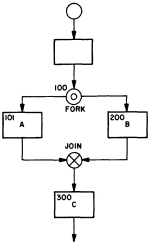
\includegraphics[width=0.25\textheight]{img/conway.pdf}

	\caption{Descripción original del modelo de \emph{fork and join}
	presentado por Melvin Conway en 1963\cite{conway1963}.}

	\label{conway}

\end{figure}

Dado que la creación de hilos suele ser una operación costosa, la mayoría de las
implementaciones de \emph{OpenMP} suelen no destruir los hilos creados durante
el \emph{fork}, sino que se mantienen inactivos para ser reutilizados cuando se
encuentre otra región de trabajo compartido.

El segundo modelo implementado en \emph{OpenMP} a partir de la versión $3.0$ es
el de tareas. En este modelo cuando se encuentra una región de trabajo
compartido, se crea un conjunto de $N$ hilos de ejecución pero no se crean
tareas para esos hilos inmediatamente. Durante le ejecución de la región de
trabajo compartido, se crean tareas que son colocadas en una cola de ejecución.
Cuando un hilo de ejecución del conjunto esta libre se le asigna una tarea de la
cola de ejecución. Cuando un hilo termina de ejecutar una tarea, toma otra de la
cola de tareas o espera. Solo se destruyen los hilos cuando se termina la
ejecución de todas las tareas y se sale de la región de trabajo compartido.

Dado que la creación de las tareas se puede hacer luego de la creación de los
hilos de ejecución, este modelo permite una mayor distribución temporal de las
tareas creadas en una región compartida. También permite que una tarea cree
nuevas tareas dentro de la misma región.

\subsubsection{Directivas de OpenMP}

Para la creación de una región de trabajo compartido bajo el modelo de tareas se
utiliza la directiva \emph{omp parallel}, y para creación de las tareas dentro
de la región se utiliza la directiva \emph{omp task}.

En el caso de \emph{OpenMP}, su uso para paralelismo de datos se realiza
comúnmente a través de la directiva \emph{parallel for}, mientras que la
directivas \emph{parallel sections} y \emph{parallel section} son utilizadas
para el paralelismo de tareas.


\chapter{Sistema propuesto}

\label{sistemaPropuesto}

% vim: set spell spelllang=es syntax=tex :

\section{Descripción del framework}

Para aumentar el throughput del sistema se aplicaran las dos técnicas discutidas
con anterioridad. En primer lugar el sistema no estará limitado a tomar solo un
cuadro por ves. La segunda optimización consta en dividir cada cuadro para que
cada parte pueda ser procesada por un thread distinto. También debe mantenerse
que las distintas pilas de plugins ejecuten de forma independiente una de la
otra.

Para esto se propone la siguiente secuencia de procesamiento para cada ítem (un
cuadro en el caso de la solución especifica para fútbol de robots):

\begin{enumerate}

\setcounter{enumi}{-1}

\item	Antes de la ejecución el usuario establece una cantidad máxima de tareas
	en ejecución simultanea.

\item	El hilo de captura genera o captura un ítem y lo deposita en el buffer.

\item	Una tarea maestra consume el ítem mas reciente del buffer y crea una
	tarea de búsqueda para su procesamiento. Si hay mas tareas que las
	permitidas o no hay ítems en el buffer, espera.

\item	Cada tarea de búsqueda crea tantas tareas por cada una de sus pilas de
	\emph{plugins}. Mientras espera a que estas taras terminen no debe ser
	contada para el limite de tareas en ejecución.

\item	Cada tarea fracciona el ítem y crea tantas tareas como fragmentos del
	ítem se hallan creado. Esta tarea terminara tan pronto como sus tareas
	hijas terminen. Mientras espera no contribuirá al limite de tareas en
	ejecución.

\item	Las tareas procesaran cada fragmento utilizando la pila de
	\emph{plugins}. Antes de terminar eliminara el fragmento del ítem.

\item	Cuando terminan todas las tareas de las pilas de plugins, la tarea de
	búsqueda resume la ejecución para eliminar el ítem de la memoria y
	posiblemente realizar tareas conteo.

\end{enumerate}

Algo que no queda especificado en la descripción anterior, es la naturaleza de
las tareas. Por un lado, las tareas pueden comenzar su ejecución al momento de
ser creadas o pueden esperar a que la cantidad de tareas en ejecución sea menor
que el máximo establecido. La primera opción tiene como desventaja que dado que
el único control sobre la cantidad de tareas se realiza al consumir un ítem, la
cantidad de tareas en ejecución sea mayor al máximo establecido durante una
porción significativa de la duración del programa. La segunda opción solo
funcionara satisfactoriamente si se asegura que la próxima tarea a ejecutar sea
la mas antigua.

El establecer un máximo de hilos en ejecución nos permite asegurarnos de que los
hilos no compitan por la CPU y que esta se mantenga ocupada siempre que haya
tareas a realizar, simplemente estableciendo tal máximo como el números de
procesadores disponibles. Es por esto que la segunda opción es la mas deseable.

Las clases del framework básico son las siguientes:

\begin{description}

\item[Item]: Esta clase define un tipo genérico de los ítems que serán tratados
	por el sistema.

\item[RingBuffer]: Este es el buffer donde se guardan los ítems generados
	mientras esperan ser procesados. El buffer guarda solo punteros a
	objetos de la clase \emph{Item} y no tiene mecanismos de control que
	permitan acceder la estructura desde múltiples threads al mismo tiempo.
	Cuando se solicita un ítem, se devuelve el puntero al mas recientemente
	agregado o \textbf{NULL} en caso de que la estructura este vacía. Cuando
	se intenta agregar un nuevo ítem pero la estructura esta llena se coloca
	este en lugar del ítem mas viejo en la estructura y se retorna el
	puntero a este al llamador, delegándole su destrucción. La destrucción
	del ítem se delega al llamador por dos motivos. El primero es que el
	buffer desconoce el tipo real del ítem. La segunda razón es que para
	poder ser utilizado de forma segura, las llamadas a los métodos del
	buffer deben estar dentro de secciones criticas y realizar las
	eliminaciones dentro de estas podría ser muy lento.

\item[Input]: Se trata de una clase que funciona como definición de la interfaz
	de las clases que generan los ítems. Sus métodos principales son
	\emph{run} y \emph{generate}. El método \emph{generate} debe ser re
	implementado por las clases hijas para generar el tipo de ítem
	especifico del sistema. El método \emph{run} es el encargado de generar
	los ítems llamando a \emph{generate} y colocarlos en el
	\emph{RingBuffer}. Este último método puede ser redefinido si la
	aplicación así lo requiere.

\item[ItemSlicer]: Es la clase que define la interfaz de las clases encargadas
	de dividir los ítems. Se definen dos métodos. El primero es \emph{slice}
	que recibe como parámetro ítem y la cantidad de partes en la que este
	debe ser dividido y retorna un arreglo de ítems. El segundo método es
	\emph{delPart} que recibe como parámetro una de las partes creadas por
	el método \emph{slice} y la elimina.

\item[Plugin]: Esta clase define una interfaz para los plugins que realizaran
	las distintas partes del procesamiento de la imagen. Solo se define el
	método \emph{process} que tiene como único parámetro un puntero a un
	objeto de la clase \emph{Item}.

\item[PluginStack]: Esta es la clase que tomara el ítem y se encarga de
	entregarlo a cada uno de los plugins. Tiene solo dos métodos,
	\emph{addPlugin}, para agregar un plugin, y \emph{process} que tiene
	como parámetro un ítem, para procesar un ítem.

\item[ItemSwitch]: Es la clase encargada de tomar los cuadros del buffer, crear
	la partición utilizando la clase descendiente de \emph{ItemSlicer},
	crear las tareas para que las partes sean procesadas por las pilas de
	plugins y crear los hilos que ejecutaran las tareas. La cantidad hilos y
	la cantidad de partes en las cuales dividirá el ítem se definirán
	durante su creación.

\end{description}

\begin{figure}[h]

	\includegraphics[width=\textwidth]{img/clasesFramework.pdf}

	\caption{Diagrama de clases Framework base.}

\end{figure}

Para adaptar el framework para utilizarlo como un sistema de visión por
computadora para el fútbol de robots se incorporaron las siguientes clases, las
cuales fueron tomadas y modificadas del sistema de visión presentado en
\cite{torres2014}:


\begin{description}

\item[Frame]: Subclase de \emph{Item}. Contiene una imagen que representa un
	cuadro y una estructura auxiliar que contiene la información necesaria
	para el funcionamiento de los plugins.

\item[CaptureFromFile]: Subclase de \emph{Input}. Es la clase encargada de crear
	el flujo de objetos \emph{Frame}, tomando cada cuadro desde un archivo
	de vídeo.

\item[FrameSlicer]: Subclase de \emph{ItemSlicer}. En este caso lo que se divide
	es la imagen del cuadro. Cada sub cuadro tendrá un solapamiento con los
	adyacente ya que se debe evitar que un robots o la pelota no este
	totalmente contenido dentro de por lo menos un sub cuadro. Para
	minimizar el área solapada las particiones se realizan de manera tal que
	se minimice el perímetro pero ocupen la mayor área posible. Para lograr
	esto se busca la partición que haga que la relación entre el alto y el
	ancho sea lo mas cercana a uno.

\item[Subclases de \emph{Plugin}]: \emph{PluginBlur},
	\emph{PluginColorConversions}, \emph{PluginColorSegmentation},
	\emph{PluginDetectBalls}, \emph{PluginFindBlobs},
	\emph{PluginFindSecondariesBlobs}, \emph{PluginMorphology} y
	\emph{PluginNetworking}.

\item[Clases auxiliares]: \emph{ball}, \emph{colorspace}, \emph{datastruct},
	\emph{homography}, \emph{marker}, \emph{pattern},
	\emph{pattern\_matching}, \emph{practicalsocket}, \emph{segmentation},
	\emph{team}, \emph{timer}.

\end{description}

\begin{figure}[h]

	\includegraphics[width=\textwidth]{img/clasesFrameworkRobots.pdf}

	\caption{Diagrama de clases Framework del framework instanciado para el
	sistema de visión para el fútbol de robots.}

\end{figure}

Existen dos parámetros ajustables. El primero es la cantidad de hilos que
ejecutaran las tareas de búsqueda. El segundo parámetro es la cantidad de partes
en las cuales se dividirá el cuadro.


\chapter{Experimentación}

\label{experimentacion}

% vim: set spell spelllang=es syntax=tex :

\section{Resultados}

Para comprobar el funcionamiento del nuevo framework se utilizaron los vídeos de
resolución 640x480, 800x600 y 1280x720, en el equipo con procesador Intel Xeon
E5-2630 con 16GiB de memoria ram.

Se realizaron pruebas con cada vídeo, variando la cantidad de partes en las que
fueron divididos los cuadros y la cantidad de cuadros procesados al mismo tiempo
entre uno y doce. Se ejecuto el programa durante 10 segundos. Se contó la
cantidad de cuadros procesados en ese tiempo y el retardo máximo la creación de
un cuadro y la finalización de su procesamiento. Cable aclarar que estas
estadísticas tienen solo en cuenta el procesamiento de los cuadros, no si se
encontraron los robots o pelota en ellos. Los resultados finales pueden verse
en las siguientes tablas.

//tablas de tiempo y retardo.

//Poner gráfico de retardo/cuadros


\chapter{Uso educativo}

\label{usoEducativo}

% vim: set spell spelllang=es syntax=tex :

\section{Uso como herramienta educativa}

\label{usoEducativo}

El sistema puede ser utilizado como herramienta educativa en varios niveles, y
tanto en materias de visión por computadora como en materias de sistemas
paralelos.

En una materia de sistemas paralelos el sistema puede cumplir varios objetivos.
Una vez introducidos los conceptos de \emph{speedup} y eficiencia el sistema
puede ser utilizado para que los alumnos puedan practicar su calculo.

\begin{enumerate}

	\item{Utilizando el sistema para procesar el vídeo de 800x600 píxeles,
		dividiéndolo el 4 fragmentos:

\begin{enumerate}

	\item{¿Cuantos cuadros por segundo se logran procesar si se utilizan 1 y
		2 hilos de búsqueda?}

	\item{Calcule el \emph{speedup} y la \emph{eficiencia} cuando se
		utilizan 2 hilos de búsqueda.}

\end{enumerate}}

\end{enumerate}

Con el fin de reforzar el concepto de eficiencia linea y no lineal, se puede
solicitar a los alumnos que realicen una predicción sobre el comportamiento del
sistema utilizando la información obtenida en los puntos anteriores. Luego de
contrastar las predicciones con los resultados reales el alumno podrían intentar
encontrar explicaciones posibles para la reducción del \emph{speedup} utilizando
sus conocimientos de arquitectura de computadoras. En las siguientes preguntas
algunos valores deberán ajustarse dependiendo de la plataforma experimental con
la que cuenten los alumnos, en estos ejemplos se considerara que cuentan con la
misma plataforma experimental que la utilizada en este trabajo.

\begin{enumerate}

	\item{[...]

\begin{enumerate}

	\setcounter{enumii}{2}

	\item{¿Cuantos cuadros por segundo estima que se procesaran
		aproximadamente si se utilizan 3, 4 y 16 hilos de búsqueda?}

	\item{Realice el experimento de procesar el vídeo con 3, 4 y 16 hilos de
		búsqueda ¿Que tan precisa fueron sus predicciones realizadas en
		el inciso anterior?}

	\item{¿Cual espera que sea el comportamiento del sistema si se utilizan
		128 hilos de búsqueda? ¿Y si se utilizan 1024?}

	\item{¿Que explicaciones posibles existen para la reducción del
		\emph{speedup}?}

	\item{Si se tiene una computadora con un procesador de 4 núcleos
		¿Cuantos hilos de búsqueda recomendaría?}

\end{enumerate}}

\end{enumerate}

Como se pudo verificar en este trabajo, la fragmentación de los datos tiene un
impacto crucial en la eficiencia de los programas paralelos. Para que los
alumnos experimenten con este concepto el sistema desarrollado es ideal, ya que
permite experimentar con distintas cantidad de hilos y cantidad de fragmentos.
Para que los alumnos puedan fortalecer este concepto proponemos como practica
que los estudiantes ejecuten el programa dividiendo el cuadro en 16, 17 y 18
partes, y luego busquen otras cantidades de divisiones donde se produzca una
caída de los \emph{FPS} con respecto a las cantidades de fragmentos inmediatas.
Con esto se espera que los alumnos puedan concluir que las cantidades de
divisiones cuyos valores son primos son perjudiciales y de esta manera
reforzar la idea de que la distribución de los datos es importante.

\begin{enumerate}
	
	\setcounter{enumi}{1}

	\item{Si se utilizan 4 hilos de búsqueda y se dividen los cuadros en 16,
		17 y 18 partes para procesar el vídeo de 1280x720 píxeles:

\begin{enumerate}

	\item{¿Cuantos cuadros por segundo procesa el sistema?}

	\item{Limitándose a una cantidad de fragmentos menor a 17 ¿Encuentra
		otros valores para los cuales el sistema tenga mayor rendimiento
		tanto si se utiliza un hilo menos o un hilo más?}

\end{enumerate}}


\end{enumerate}

Una vez que los alumnos tienen incorporados los conceptos de \emph{speedup},
eficiencia, y la importancia de la distribución de los datos, proponemos que
experimenten con distintas configuraciones de ejecución con el fin de que el
sistema cumpla con requerimientos específicos de tiempo de procesamiento y
\emph{FPS}. Con ésto se espera que los estudiantes incorporen la noción de que
distintas aplicaciones pueden tener distintos requerimientos específicos que
deben ser tenidos en cuenta al momento de configurarla.

\begin{enumerate}

	\setcounter{enumi}{2}

	\item{Utilizando el sistema para procesar el vídeo de 800x600 píxeles:

\begin{enumerate}

	\item{Si se utilizan 12 hilos de búsqueda ¿En cuantos fragmentos deberán
		dividirse los cuadros para que la cantidad de cuadros por
		segundo procesados sea mayor a 180?}

	\item{Si se utilizan 12 hilos de búsqueda ¿En cuantos fragmentos deberán
		dividirse los cuadros para que el retardo del cuadro sea menor a
		6 centésimas de segundo?}

	\item{Si se divide el cuadro en 15 fragmentos ¿Cuantos hilos de búsqueda
		se deberán usar para que la cantidad de cuadros por segundo
		procesados sea mayor a 180?}

\end{enumerate}}

\end{enumerate}

Finalmente si se desea utilizar el sistema con la finalidad de que los alumnos
realicen practica de programación de sistemas paralelos, se puede plantear como
ejercicio la optimización del pluguin de \emph{segmentación de color} utilizando
instrucciones escalares.

\begin{enumerate}

	\setcounter{enumi}{3}

	\item{Modifique el plaguin de \emph{segmentacion de color} utilizando
	instrucciones vectoriales ¿Cual es la mejora obtenida?}

\end{enumerate}

Para las materias de visión por computadora se puede hacer uso de la facilidad
de extinción del sistema. Los alumnos pueden usar el sistema como base para la
la implementación de nuevos mecanismos para detectar los robots, pelota, o
nuevos objetos, esto implicaría la creación de nuevos plugins y pilas de
plugins.

\begin{enumerate}

	\item{Para incrementar la detección de infracciones en los partidos de
		la \emph{SSL} se desea agregar un referí a la cancha. Éste es un
		robot similar a los jugadores que proveerá una vista a nivel del
		suelo, se moverá por toda la cancha, y lleva un parche
		cuadriculado blanco y negro. Implemente una nueva pila de
		plugins para la detección del referí.}

\end{enumerate}

También se puede plantear como trabajo adaptar el framework para un dominio
distinto.

\begin{enumerate}

	\item{Utilizando como base el framework, implemente un sistema capaz de
		detectar la presencia un marcador de realidad aumentada, su
		poción y orientación con respecto a la cámara, y lo remplace por
		el logo de la \texttt{Universidad Nacional del Comahue} (con la
		orientación correspondiente). El vídeo resultante debe tener un
		retardo menor a un segundo. Puede diseñar su propio marcador de
		realidad aumentada, aunque se recomienda utilizar uno estándar.}

\end{enumerate}


\chapter{Conclusiones y trabajos futuros}

\label{conclucionesYTrabajosFuturos}

% vim: set spell spelllang=es syntax=tex :

\section{Conclusiones finales}

\label{concluciones}

En este trabajo se ha presentado un nuevo sistema de visión global por
computadora para el fútbol de robots de la \emph{SSL}, que puede ser utilizado
como herramienta educativa en una asignatura de visión por Computadora y permite
explorar distintas estrategias de paralelización. El sistema procesa cuadros de
vídeo y reporta la posición y orientación de los robots y la posición de la
pelota en cada uno de ellos.

Se describieron dos estrategias de paralelización que son aplicadas en conjunto.
Una de ellas explota el paralelismo dentro de cada cuadro, dividiendo los
cuadros en fragmentos que son procesados de forma independiente. La otra
estrategia se basa en el procesamiento simultáneo de diferentes cuadros del
vídeo (independientes unos de otros).

Se realizó una implementación en \emph{OpenMP} para \emph{C++}, basada en
plugins para facilitar su modificación en un ambiente educativo. Se detallaron
las tareas que ejecuta el sistema para implementar las estrategias de
paralelización. Se estudió el comportamiento del sistema en términos de
\emph{FPS} y de retardo en el procesamiento de los cuadros para diferentes
configuraciones del sistema en distintas resoluciones de vídeo.

En un servidor con un procesador Intel Xeon E5-2630 (6 cores y multithreading
simultáneo) el software es capas de procesar un vídeo de 800x600 píxeles de
resolución a una taza de 196 cuadros por segundo y un vídeo de 1280x720 píxeles
resolución a una taza de 135 cuadros por segundo.

Se pudo comprobar como un numero primo de fragmentos afectaba de forma negativa
el desempeño del sistema, y como un bajo numero de estos obliga a los hilos a
competir por los recursos de caché.

El framework final es adaptable a distintos dominios y su arquitectura basada en
plugins permite modificarlos y agregar nuevos fácilmente. Finalmente,
modificando las variables de cantidad de fragmentos e hilos de búsqueda el
sistema puede adaptarse a un amplio rango de configuraciones de hardware.

\section{Trabajos futuros}

\label{trabajosFuturos}

Si bien el sistema funciona correctamente, existen aspectos que hacen difícil su
aplicación como remplazo para los sistemas de visión global utilizados hoy en
día en las competencias de la \emph{SSL}. En la implementación actual, si se
desea calibrar los colores de los parches o la pelota se deben realizar
modificaciones en el código. Seria deseable una interfaz gráfica que permita
modificar estos datos interactivamente. Seria útil también mostrar gráficamente
la detección de los objetos.

La taza decrecimiento del \emph{speedup} se vio disminuida a partir de los seis
hilos de búsqueda, para analizar si la causa se debe a que los accesos a memoria
crean un cuello de botella o si se se debe a que con seis hilos se alcanza un
alto paralelismo a nivel de instrucción se podría analizar la cantidad de
instrucciones por ciclo.

Como trabajo futuro se planea hacer una interfaz de usuario gráfica para
configurar el sistema. Además, se cree conveniente implementar soluciones
paralelas optimizadas de los plugins para utilizar el sistema en competencias de
fútbol de robots, para esto es aconsejable encontrar la causa de la reducción
del crecimiento del \emph{speedup} analizando la cantidad de instrucciones por
ciclo.


% vim: set spell spelllang=es syntax=tex :

\appendix
\clearpage
\addappheadtotoc
\appendixpage

\chapter{Publicaciones derivadas}

\begin{figure}[!htb]

	\centering
	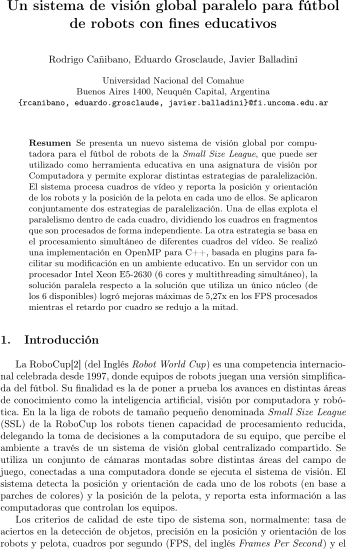
\includegraphics[width=0.6\textwidth]{img/cacic2016-robocup.pdf}
	\caption*{Primera hoja de la publicación ``Un sistema de visión global
	paralelo para fútbol de robots con fines educativos''.}

\end{figure}


\bibliographystyle{babplain}

\bibliography{biblio}

\end{document}
